\documentclass[tikz,border=8pt]{standalone}
% Requer xelatex e a fonte Poppins. Ajuste o Path abaixo (ou use \setmainfont{Poppins} se ela estiver instalada).
\usepackage{fontspec}
\setmainfont{Poppins}[Path=/usr/share/fonts/truetype/google-fonts/,Extension=.ttf,UprightFont=*-Regular,BoldFont=*-Bold,ItalicFont=*-Italic,BoldItalicFont=*-BoldItalic]
\usepackage{xcolor}
\definecolor{azulescuro}{HTML}{4A6F9C}
\definecolor{azulmedio}{HTML}{6F93BC}
\definecolor{azulclaro}{HTML}{E9EDF3}
\definecolor{azulsenac}{HTML}{1F4E9A}
\definecolor{laranja}{HTML}{F19E37}
\definecolor{laranjaescuro}{HTML}{D9731A}
\definecolor{laranjaclaro}{HTML}{FDEFD9}
\definecolor{cinzatitulo}{HTML}{333333}
\definecolor{cinzatexto}{HTML}{5C5C5C}
\usepackage{tikz}
\usetikzlibrary{positioning,arrows.meta,fit,backgrounds,calc}

\begin{document}
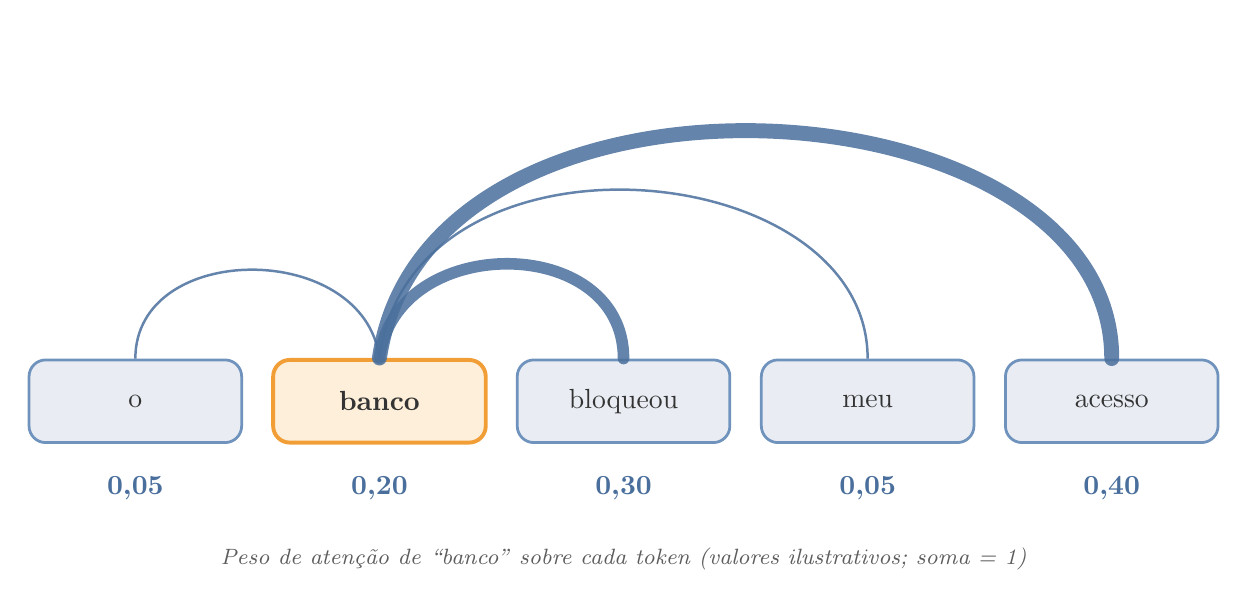
\begin{tikzpicture}[font=\small\color{cinzatexto},
  tok/.style={draw=azulmedio, fill=azulclaro, line width=1pt, rounded corners=6pt, minimum width=2.7cm, minimum height=1.05cm, font=\normalsize\color{cinzatitulo}},
  alvo/.style={tok, draw=laranja, fill=laranjaclaro, line width=1.4pt, font=\normalsize\bfseries\color{cinzatitulo}},
  peso/.style={font=\normalsize\bfseries\color{azulescuro}}]
\def\dx{3.1}
\node[tok]  (t0) at (0*\dx,0) {o};
\node[alvo] (t1) at (1*\dx,0) {banco};
\node[tok]  (t2) at (2*\dx,0) {bloqueou};
\node[tok]  (t3) at (3*\dx,0) {meu};
\node[tok]  (t4) at (4*\dx,0) {acesso};
\node[peso] at (0*\dx,-1.1) {0,05};
\node[peso] at (1*\dx,-1.1) {0,20};
\node[peso] at (2*\dx,-1.1) {0,30};
\node[peso] at (3*\dx,-1.1) {0,05};
\node[peso] at (4*\dx,-1.1) {0,40};
% arcos a partir de "banco"; espessura proporcional ao peso
\draw[azulescuro, line width=0.9pt,  opacity=0.85] (t1.north) .. controls +(-0.2,1.5) and +(0,1.5) .. (t0.north);
\draw[azulescuro, line width=4.2pt,  opacity=0.85, line cap=round] (t1.north) .. controls +(0.2,1.6) and +(0,1.6) .. (t2.north);
\draw[azulescuro, line width=0.9pt,  opacity=0.85] (t1.north) .. controls +(0.4,3.1) and +(0,2.6) .. (t3.north);
\draw[azulescuro, line width=5.4pt,  opacity=0.85, line cap=round] (t1.north) .. controls +(0.6,4.1) and +(0,3.6) .. (t4.north);
\node[font=\footnotesize\itshape\color{cinzatexto}] at (2*\dx,-2.0) {Peso de atenção de “banco” sobre cada \textit{token} (valores ilustrativos; soma = 1)};
\end{tikzpicture}
\end{document}
